\documentclass[12pt]{article}
\usepackage[a4paper, margin=2.5cm]{geometry}
\usepackage{booktabs}
\usepackage{graphicx}
\usepackage{caption}
\usepackage{subcaption}
\usepackage{amsmath}
\usepackage{array}
\usepackage{multirow}
\usepackage{xcolor}
\usepackage{hyperref}
\usepackage{siunitx}
\usepackage{microtype}

\hypersetup{colorlinks=true, linkcolor=blue, citecolor=blue, urlcolor=blue}

%% Supplementary numbering: S1, S2, ...
\renewcommand{\thefigure}{S\arabic{figure}}
\renewcommand{\thetable}{S\arabic{table}}
\setcounter{figure}{0}
\setcounter{table}{2}

\captionsetup{font=small, labelfont=bf}

\title{\textbf{Supplementary Material}\\[0.6em]
\large Deep Learning Architectures for Brain Tumor MRI Classification:\\
Systematic Comparison with a Novel Hybrid CNN-Transformer,\\
Explainable AI and Statistical Significance Testing}
\author{Balasis Ioannis \and Makris Christos}
\date{}

\begin{document}
\maketitle


%% ═══════════════════════════════════════════════════════════════════════════
%% FIGURE S1 — Confusion Matrices
%% ═══════════════════════════════════════════════════════════════════════════
\section*{Figure S1 — Confusion Matrices (503-Sample Tumour-Positive Subset)}

\begin{figure}[ht]
  \centering
  \begin{subfigure}[t]{0.32\textwidth}
    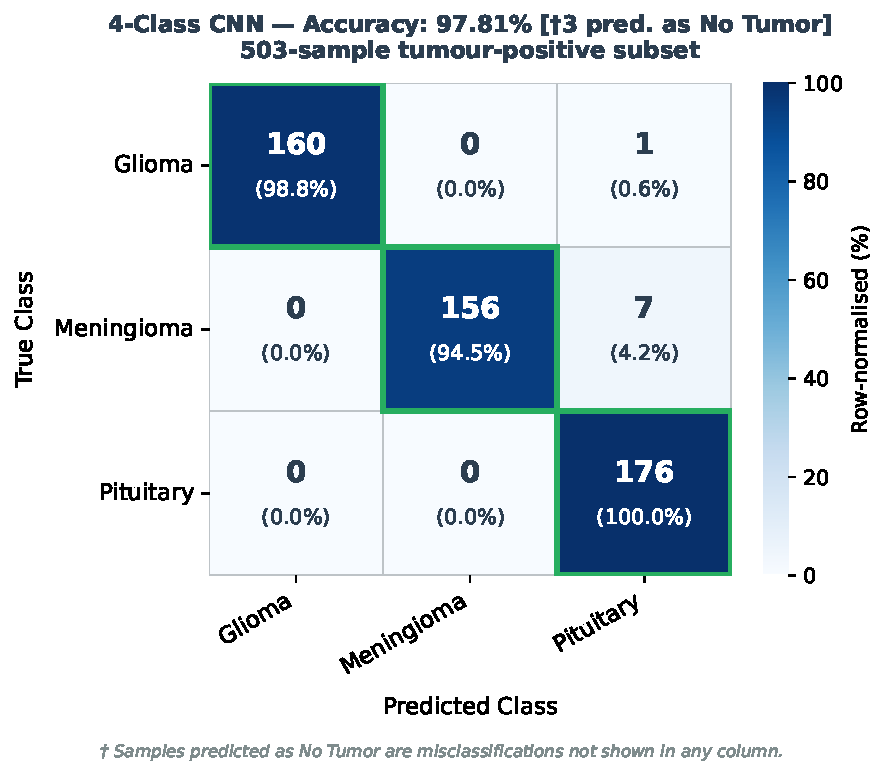
\includegraphics[width=\textwidth]{confusion_matrices_503/cm_4class_cnn_503}
    \caption{4-Class CNN}
  \end{subfigure}\hfill
  \begin{subfigure}[t]{0.32\textwidth}
    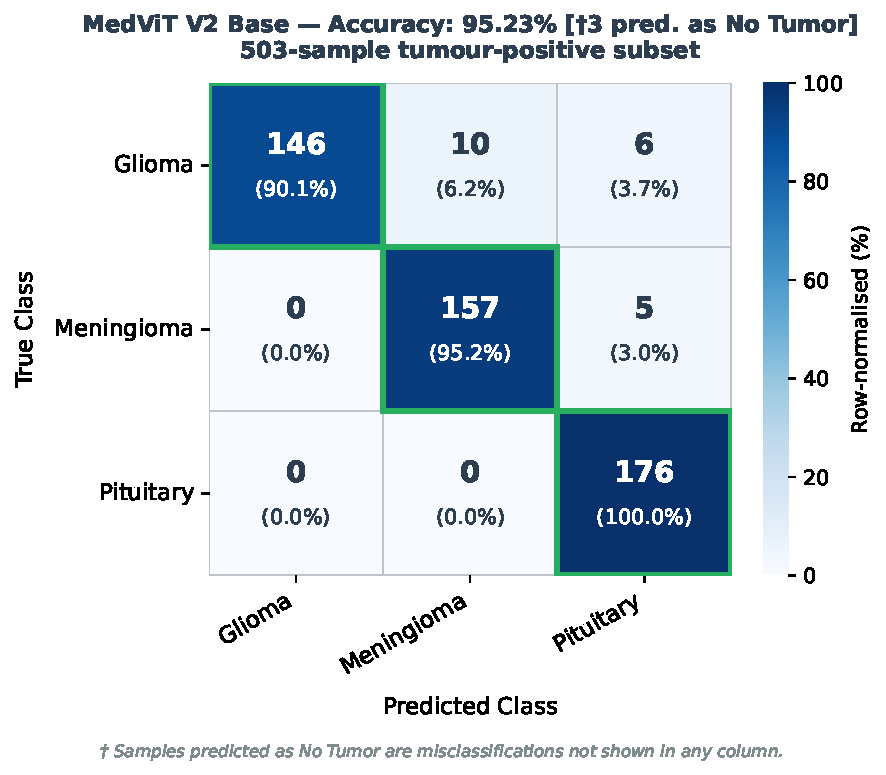
\includegraphics[width=\textwidth]{confusion_matrices_503/cm_medvit_base_503}
    \caption{MedViT~V2 Base}
  \end{subfigure}\hfill
  \begin{subfigure}[t]{0.32\textwidth}
    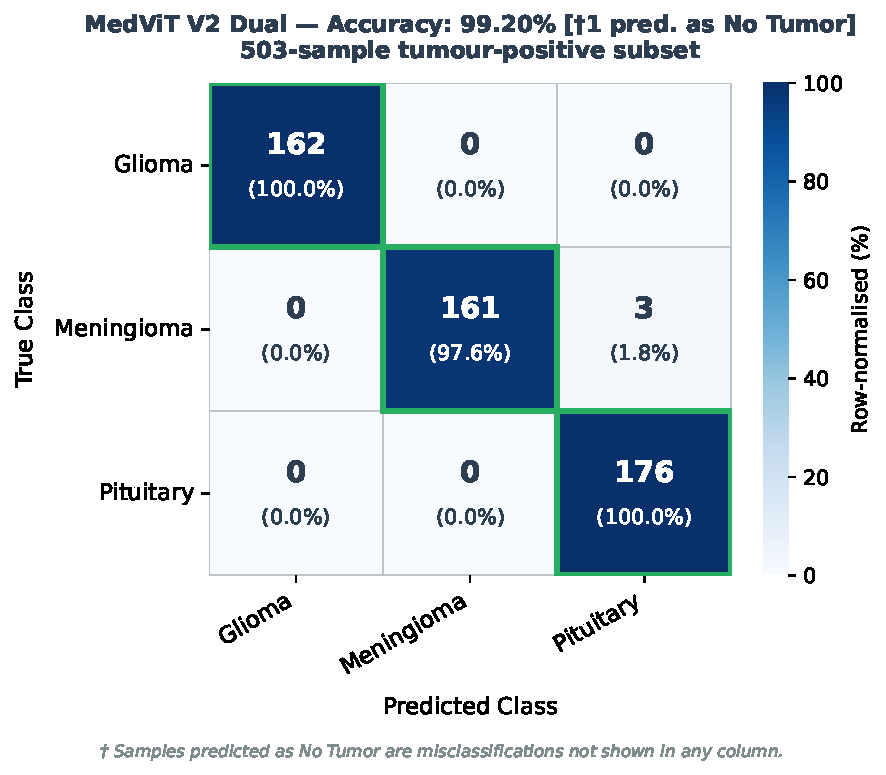
\includegraphics[width=\textwidth]{confusion_matrices_503/cm_medvit_dual_503}
    \caption{MedViT~V2 Dual}
  \end{subfigure}
  \caption{Row-normalised confusion matrices on the 503-sample tumour-positive
    evaluation subset (Glioma: 162, Meningioma: 165, Pituitary: 176) for the
    three four-class architectures. No~Tumour samples are excluded from this
    subset to enable fair cross-model comparison (the 3-Class~CNN and 1-vs-1
    Ensemble architectures cannot predict No~Tumour). Diagonal cells (green
    border) show correct classifications; off-diagonal cells show
    misclassifications. Counts and row-normalised percentages are both
    displayed. The number of tumour-positive samples incorrectly predicted as
    No~Tumour by each model is reported in the figure sub-title (4-Class~CNN: 3,
    MedViT~V2~Base: 3, MedViT~V2~Dual: 1).}
  \label{fig:s1_confusion}
\end{figure}

\newpage


%% ═══════════════════════════════════════════════════════════════════════════
%% FIGURE S2 — Wilcoxon Heatmap
%% ═══════════════════════════════════════════════════════════════════════════
\section*{Figure S2 — Pairwise Wilcoxon Signed-Rank Test with Bonferroni Correction}

\begin{figure}[ht]
  \centering
  \includegraphics[width=0.85\textwidth]{statistical_analysis_results/wilcoxon_heatmap}
  \caption{Pairwise Bonferroni-adjusted $p$-values from the Wilcoxon signed-rank
    test across all 36 pairs of the nine architectures, computed on the
    503-sample tumour-positive evaluation subset. Each cell shows the adjusted
    $p$-value; cells with $p_{\text{Bonf}} < 0.05$ are shaded darker,
    indicating statistically significant pairwise differences. The overall
    Friedman test yielded $\chi^2_F(8) = 164.45$, $p < 0.001$, confirming
    significant variation in performance across architectures. Pairwise
    Bonferroni-adjusted Wilcoxon signed-rank tests reveal, however, that
    differences among the top-performing architectures are not statistically
    significant after correction for multiple comparisons (e.g.\
    $p_{\text{Bonf}} = 0.240$ for MedViT~V2~Dual vs.\ Binary~CNN).
    Full results are reported in Section~3.2 of the main paper.}
  \label{fig:s2_wilcoxon}
\end{figure}

\newpage


%% ═══════════════════════════════════════════════════════════════════════════
%% TABLE S3 — 5-Fold Cross-Validation Results
%% ═══════════════════════════════════════════════════════════════════════════
\section*{Table S3 — 5-Fold Stratified Cross-Validation Results}

\begin{table}[ht]
\centering
\caption{Per-fold validation accuracy (\%) from 5-fold stratified cross-validation
  on the training+validation set (90\% of full dataset, \texttt{random\_state=42}).
  The frozen 10\% test set was never used during cross-validation.
  \textbf{CV Test Acc} = accuracy of the CV final model on the full 703-sample
  test set (all four classes including No~Tumour).
  This differs from Table~1 of the main paper for two reasons: (1)~the CV
  final model is retrained from scratch on the full train+val set for a fixed
  number of epochs equal to the median best epoch across folds, without
  further early-stopping optimisation; (2)~it is evaluated on all 703 test
  samples, whereas Table~1 uses the 503-sample tumour-positive subset to
  enable fair cross-model comparison.
}
\label{tab:s3_cv}
\begin{tabular}{lcccc}
\toprule
\textbf{Fold} &
\textbf{4-Class CNN} &
\textbf{3-Class CNN} &
\textbf{Binary CNN} &
\textbf{Multi-Dual System} \\
\midrule
1 & 97.39 & 97.12 & 99.53 & 98.10 \\
2 & 98.18 & 97.01 & 99.84 & 98.10 \\
3 & 98.10 & 98.12 & 99.68 & 96.76 \\
4 & 98.02 & 98.01 & 99.45 & 97.78 \\
5 & 98.26 & 98.34 & 98.89 & 98.18 \\
\midrule
\textbf{CV Mean (\%)}      & 97.99 & 97.72 & 99.48 & 97.78 \\
\textbf{CV Std (\%)}       &  0.31 &  0.54 &  0.32 &  0.53 \\
\midrule
\textbf{CV Test Acc (\%)}  & 90.90 & 93.24 & 95.16 & 97.44 \\
\bottomrule
\end{tabular}
\end{table}

\vspace{1em}
\noindent\textit{Note.} Cross-validation used \texttt{StratifiedKFold}
($k=5$, \texttt{shuffle=True}, \texttt{random\_state=42}) as in Dem\v{s}ar (2006).
Each fold's accuracy is the best validation accuracy before early stopping
(\texttt{patience=15}). The final model is retrained on the full train+val
set for the median best epoch across folds.
The \textbf{per-fold CV Mean} values are the primary cross-validation results
reported in the main paper; \textbf{CV Test Acc} is a secondary diagnostic
showing the generalisability of the CV final model and is \emph{not} intended
for direct comparison with Table~1, which reports the original trained models
evaluated on the 503-sample tumour-positive subset.

\newpage


%% ═══════════════════════════════════════════════════════════════════════════
%% TABLE S4 — Bootstrap CI Occlusion Confidence Drops
%% ═══════════════════════════════════════════════════════════════════════════
\section*{Table S4 — Bootstrap Confidence Intervals for Occlusion Confidence Drops}

\begin{table}[ht]
\centering
\caption{Bootstrap confidence intervals (95\%, $B=10{,}000$ iterations) for
  Grad-CAM occlusion confidence drops across three tumour classes for the five
  architectures on which Grad-CAM is applicable.
  \emph{Occlusion confidence drop} = reduction in softmax confidence when the
  Grad-CAM saliency region is masked to zero, as a percentage of baseline
  confidence. $n$ = number of correctly classified test samples used.
  Meningioma 95\% CIs do not overlap with Glioma or Pituitary CIs in any
  model, confirming a statistically significant difference in saliency
  localisation difficulty (Meningioma Paradox, Section~3.3).}
\label{tab:s4_bootstrap}
\begin{tabular}{llccccc}
\toprule
\textbf{Model} & \textbf{Class} &
\textbf{Mean (\%)} & \textbf{Std (\%)} &
\textbf{CI$_{2.5}$ (\%)} & \textbf{CI$_{97.5}$ (\%)} &
$n$ \\
\midrule
\multirow{3}{*}{4-Class CNN}
  & Glioma      &  5.8 & 15.3 &  3.6 &  8.3 & 160 \\
  & Meningioma  & 64.1 & 37.2 & 58.1 & 69.9 & 156 \\
  & Pituitary   &  1.3 &  8.7 &  0.3 &  2.8 & 176 \\
\midrule
\multirow{3}{*}{3-Class CNN}
  & Glioma      & 11.0 & 23.2 &  7.6 & 14.7 & 161 \\
  & Meningioma  & 45.8 & 40.4 & 39.5 & 52.0 & 162 \\
  & Pituitary   &  6.0 & 11.3 &  4.4 &  7.8 & 175 \\
\midrule
\multirow{3}{*}{Multi-Dual System}
  & Glioma      &  8.8 & 25.0 &  5.2 & 13.0 & 156 \\
  & Meningioma  & 51.7 & 41.2 & 45.0 & 58.3 & 147 \\
  & Pituitary   &  1.8 & 10.9 &  0.4 &  3.6 & 176 \\
\midrule
\multirow{3}{*}{MedViT~V2 Base}
  & Glioma      & 16.7 & 27.8 & 12.5 & 21.4 & 147 \\
  & Meningioma  & 51.1 & 34.5 & 45.7 & 56.6 & 157 \\
  & Pituitary   & 13.8 & 23.1 & 10.6 & 17.2 & 176 \\
\midrule
\multirow{3}{*}{MedViT~V2 Dual}
  & Glioma      &  2.1 &  9.2 &  0.9 &  3.7 & 162 \\
  & Meningioma  & 66.7 & 39.7 & 60.6 & 72.7 & 161 \\
  & Pituitary   &  0.6 &  6.7 &  0.1 &  1.6 & 176 \\
\bottomrule
\end{tabular}
\end{table}

\vspace{1em}
\noindent\textit{Note.} Bootstrap resampling ($B=10{,}000$, with replacement)
was applied to correctly-classified test samples per model per class.
The 95\% CI is the interval between the 2.5th and 97.5th percentiles
of the bootstrap distribution.
MedViT~V2~Base shows elevated drops for Glioma (16.7\%) and Pituitary
(13.8\%) compared with CNN models (1--11\%), consistent with the more
uniform global attention of the transformer architecture.
MedViT~V2~Dual corrects this dispersion (Glioma 2.1\%, Pituitary 0.6\%)
but concentrates the highest Meningioma drop across all models (66.7\%),
reinforcing the Meningioma Paradox.
The 1-vs-1 Ensemble is excluded as Grad-CAM is not directly applicable
to multi-model voting ensembles.

\end{document}
